\documentclass[12pt]{report}
\usepackage{scribe,graphicx,graphics}
\usepackage{subcaption}


\course{MIT 22.213} 	
\coursetitle{Nuclear Reactor Kinetics}	
\semester{Spring 2015}
\lecturenumber{2}	
\lecturedate{}		


% Insert your name here!
\scribe{Geoffrey Gunow}

\begin{document}
	
	
	\maketitle
	
	\paragraph{Intro: Code Design}
	In this problem set, I solve the neutron diffusion problem with a Python code structure using Scipy and Numpy libraries. The solver is constructed to deal with \textit{arbitrary mesh spacing} and an \textit{arbitrary group structure}. In this problem set, my code creates \textbf{dense} matrices. If sparse matrices were implemented, the runtime would be much improved. However, my goal for this problem set was to create easily readable and understandable code that can easily be translated into a faster programming language such as C/C++. In future assignments I will translate the code, implementing my own sparse matrix solvers to increase computational efficiency.
	
	\paragraph{Part A: Difference Equations}
	When solving steady-state problems in neutron diffusion, the first step is to setup matrices of the form:
	\begin{equation}
	A \phi = \frac{1}{k} F \phi
	\label{eq::matrix}
	\end{equation}
	where $k$ is the eigenvalue, $A$ is the loss matrix, $F$ is the fission source matrix, and $\phi$ is the scalar flux solution vector. The equations represented in neutron diffusion with no external source take the form:
	\begin{equation}
	- \nabla D_g(\vec{r}) \nabla \phi_g(\vec{r}) + \Sigma_{r,g}(\vec{r}) \phi_g(\vec{r}) = \frac{\chi_g(\vec{r})}{k} \sum_{g'=1}^{G} \nu \Sigma_{f,g'}(\vec{r}) \phi_{g'}(\vec{r}) + \sum_{g'\neq g} \Sigma_{s}^{g' \rightarrow g}(\vec{r}) \phi_{g'}(\vec{r}).
	\end{equation}
	The variable definitions are shown in Table~\ref{tab::diff_vars}. Note that the removal cross-section is the sum of the absorption cross-section and the outscatter cross-section.
	
	\begin{table}[ht]
		\begin{center}
			\caption{\label{tab::diff_vars} Diffusion equation variables}
			\begin{tabular}{ll}
				\hline
				Variable & Description \\
				\hline
				$\vec{r}$ & Position vector \\
				$D_g$ & Diffusion coefficient for group $g$ \\
				$\phi_g$ & Neutron flux for group $g$ \\
				$\Sigma_{r,g}$ & Removal cross-section for group $g$ \\
				$\chi_g$ & Probability that a neutron is generated in group $g$ \\
				$\nu$ & Average number of neutrons born per fission \\
				$\Sigma_{f,g'}$ & Fission cross-section for group $g$ \\
				$\Sigma_{s}^{g' \rightarrow g}$ & Cross-section for scattering from group $g'$ to $g$ \\
				\hline
			\end{tabular}
		\end{center}
	\end{table}
	
	For generality, I structured my code to account for an arbitrary number of energy groups. With a simple structured mesh, most terms can easily be transformed into the analogous spatially discretized form. The greatest difficulty lies in determining the spatially discretized form of
	\begin{equation}
	- \nabla D_g(\vec{r}) \nabla \phi_g(\vec{r}).
	\end{equation}
	Our first realization is that this can be re-written in terms of the neutron current $J$ as
	\begin{equation}
	\nabla J_g(\vec{r}).
	\end{equation}
	For one-dimensional problems we can reduce $\vec{r}$ to the one-dimensional distance $x$. This means that our problem can be reduced to 
	\begin{equation}
	\frac{d}{dx} J_g(x) + \Sigma_{r,g}(x) \phi_g(x) = \frac{\chi_g(x)}{k} \sum_{g'=1}^{G} \nu \Sigma_{f,g'}(x) \phi_{g'}(x) + \sum_{g'\neq g} \Sigma_{s}^{g' \rightarrow g}(x) \phi_{g'}(x).
	\end{equation}
	
	With a spatial mesh imposed on the problem, we can calculate the derivative using the central difference approximation to the derivate as
	\begin{equation}
	\frac{d}{dx} J_g(x) \Bigr|_{x=x_i}	\approx \frac{J_i^+ - J_i^-}{\Delta_i}
	\end{equation}
	for mesh cell $i$ with width $\Delta_i$, midpoint $x_i$, right surface current $J_{i+1/2}$ and left surface current $J_{i-1/2}$.  With this approximation, we can re-write our balance equation in terms of discretized mesh as
	\begin{equation}
	\frac{J_{i+1/2} - J_{i-1/2}}{\Delta_i} + \Sigma_{r,i,g} \phi_{g,i} = \frac{\chi_{g,i}}{k} \sum_{g'=1}^{G} \nu \Sigma_{f,g',i} \phi_{g',i} + \sum_{g'\neq g} \Sigma_{s,i}^{g' \rightarrow g} \phi_{g',i}
	\end{equation}
	where $i$ refers to mesh cell number. To clean-up the equations, we multiply through by $\Delta_i$ yielding
	\begin{equation}
	J_{i+1/2} - J_{i-1/2} + \Sigma_{r,i,g} \phi_{g,i} \Delta_i = \frac{\chi_{g,i}}{k} \sum_{g'=1}^{G} \nu \Sigma_{f,g',i} \phi_{g',i} \Delta_i + \sum_{g'\neq g} \Sigma_{s,i}^{g' \rightarrow g} \phi_{g',i} \Delta_i.
	\end{equation}
	
	Now a relation need to be found between $J_{i+1/2}$ and $J_{i-1/2}$ and the scalar flux. In general, the currents can be related to the scalar flux by demanding that at the interface between two cells the current is continuous. When the cells have constant material properties, this yields:
	\begin{eqnarray}
	J_s^- = -D_{g,i} \frac{d}{dx} \phi_g(x) \bigr|_{s} \approx -D_{g,i} \frac{\phi_{g,s} - \phi_{g,i}}{\Delta_i/2} \\
	J_s^+ = -D_{g,i+1} \frac{d}{dx} \phi_g(x) \bigr|_{s} \approx -D_{g,i+1} \frac{\phi_{g,i+1} - \phi_{g,s}}{\Delta_{i+1}/2}
	\end{eqnarray}
	where $s$ refers to the surface between the two adjacent cells. $J_s^-$ is the estimate of the current from the left cell flux, and $J_s^+$ is the estimate of the current from the right cell flux. If we equate these two estimates, we can solve for the scalar flux $\phi_{g,s}$ at the interface the two cells, yielding
	\begin{equation}
	\phi_{g,s} = \frac{D_{g,i} \phi_{g,i}\Delta_{i+1} + D_{g,i+1}\phi_{g,i+1} \Delta_i}{D_{g,i} \Delta_{i+1} + D_{g,i+1} \Delta_i}.
	\end{equation}
	
	Inserting this estimate back into our previous equations, we find
	\begin{equation}
	J_s^- = \frac{-2 D_{g,i} D_{g,i+1} (\phi_{g,i} - \phi_{g,i+1})}{D_{g,i} \Delta_{i+1} + D_{g,i+1} \Delta_i}
	\end{equation}
	
	Note that $J_s^- = J_s^+ = J_{g,i+1/2}$. This means that we can define
	\begin{equation}
	J_{i+1/2} = -\hat{D}_{g,i,i+1} (\phi_{g,i+1} - \phi_{g,i})
	\end{equation}
	where
	\begin{equation}
	\hat{D}_{g,i,i+1} = \frac{2 D_{g,i} D_{g,i+1}}{D_{g,i} \Delta_{i+1} + D_{g,i+1} \Delta_i}.
	\end{equation}
	
	This transforms our balance equation to
	\begin{align}
	-\hat{D}_{g,i-1,i} \phi_{g,i-1} + \left( \Sigma_{r,i,g} \Delta_i + \hat{D}_{g,i-1,i} + \hat{D}_{g,i,i+1} \right) \phi_{g,i} - \hat{D}_{g,i,i+1} \phi_{g,i+1} = \nonumber\\
	\frac{\chi_{g,i}}{k} \sum_{g'=1}^{G} \nu \Sigma_{f,g',i} \phi_{g',i} \Delta_i + \sum_{g'\neq g} \Sigma_{s,i}^{g' \rightarrow g} \phi_{g',i} \Delta_i.
	\end{align}
	
	In matrix form, all the terms on the left hand side of the equation belong to matrix $A$ and all the terms on the right hand side of the equation belong to matrix $F$. For the two group case with no upscatter and all neutrons born in the fast group, the two group equations form very recognizable matrix structures. When the solution vector is organized with energy groups on the outside, the matrix structure is that shown in Fig.~\ref{fig::groups_outside}. 
	\begin{figure}[ht]
		\centering
		\begin{subfigure}{.5\textwidth}
			\centering
			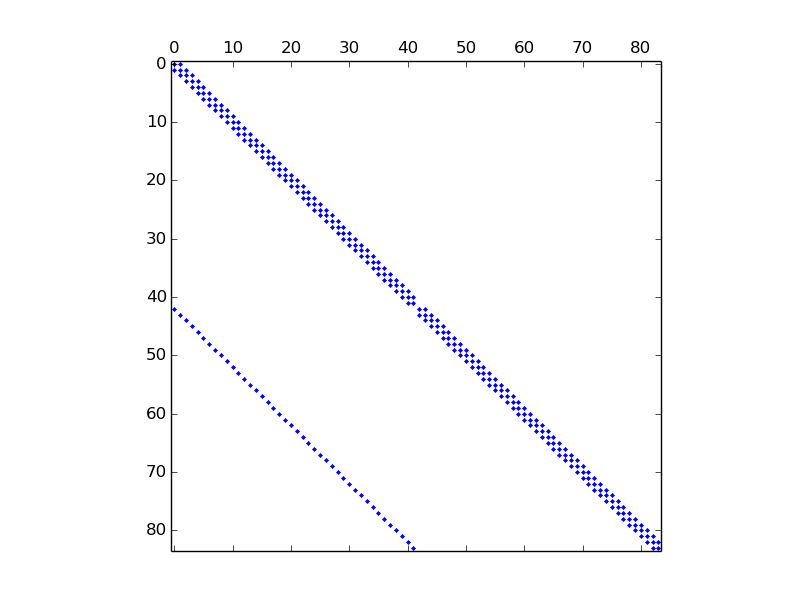
\includegraphics[width=.9\linewidth]{A_go.png}
			\caption{$A$ Matrix}
			\label{fig:A_go}
		\end{subfigure}%
		\begin{subfigure}{.5\textwidth}
			\centering
			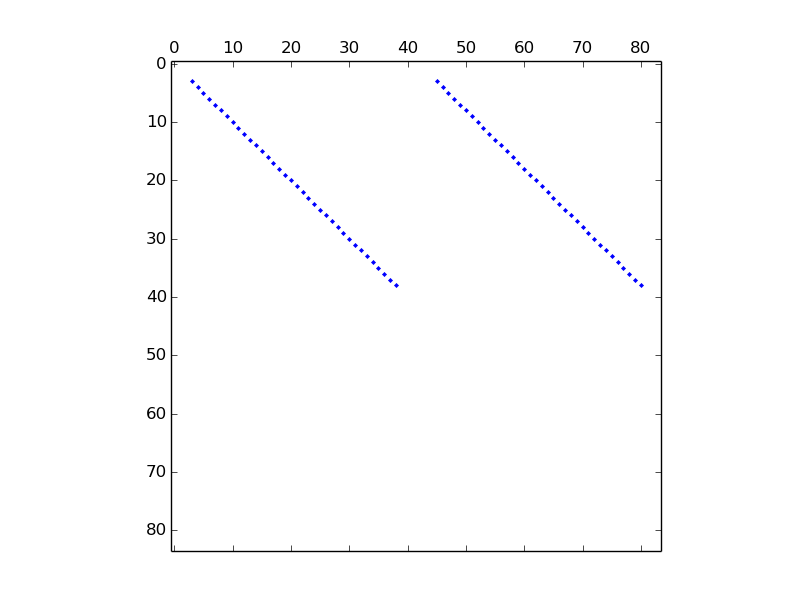
\includegraphics[width=.9\linewidth]{F_go.png}
			\caption{$F$ Matrix}
			\label{fig:F_go}
		\end{subfigure}
		\caption{Matrix structure with energy groups on the outside.}
		\label{fig::groups_outside}
	\end{figure}
	
	
	Alternatively, when energy groups are placed on the inside the non-zero elements are much closer together in the matrix. This is shown in Fig.~\ref{fig::groups_inside}.
		\begin{figure}[ht]
			\centering
			\begin{subfigure}{.5\textwidth}
				\centering
				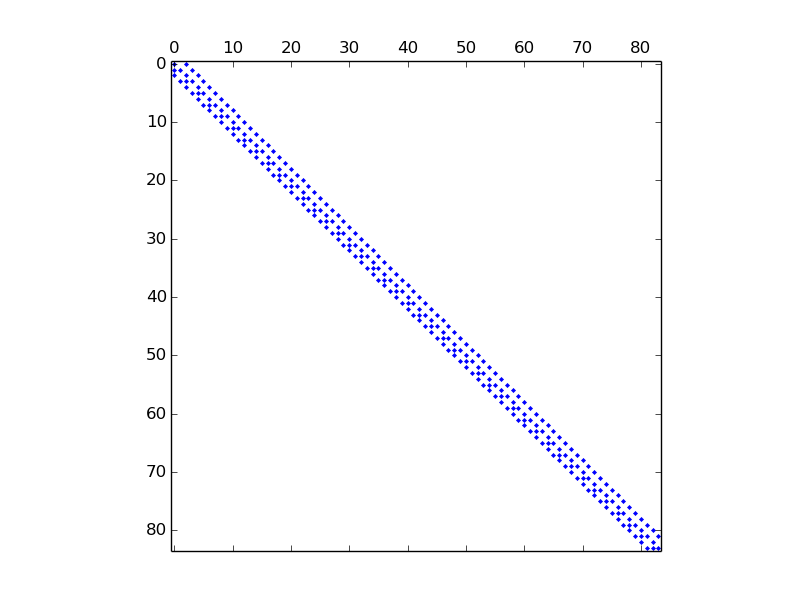
\includegraphics[width=.9\linewidth]{A_gi.png}
				\caption{$A$ Matrix}
				\label{fig:A_gi}
			\end{subfigure}%
			\begin{subfigure}{.5\textwidth}
				\centering
				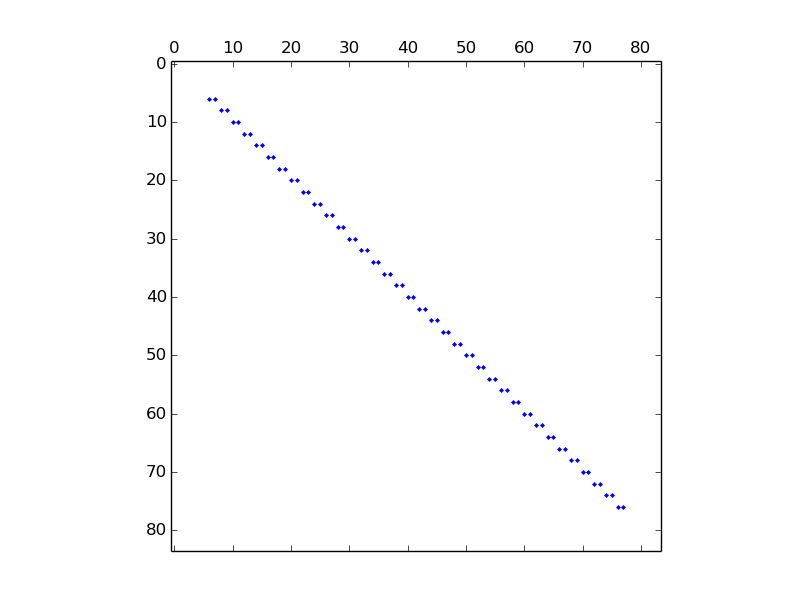
\includegraphics[width=.9\linewidth]{F_gi.png}
				\caption{$F$ Matrix}
				\label{fig:F_gi}
			\end{subfigure}
			\caption{Matrix structure with energy groups on the inside.}
			\label{fig::groups_inside}
		\end{figure}
		
	\newpage
	\paragraph{Part B: Spatial Convergence}
	When solving the neutron diffusion equation, a sufficiently fine mesh spacing is required to converge neutron flux gradients. To investigate the required mesh spacing, we consider two cases: a rodded and an unrodded 1D reactor core. This 1D representation of a reactor problem has three fuel regions surrounded by a water region with reflected boundary conditions. The middle fuel region is chosen to have a higher absorption cross-section in the rodded case. The resulting flux profiles are shown in Fig.~\ref{fig::flux_profiles} for both the rodded and unrodded cores. Note that in these plots the flux is normalized such that the average fission rate across nodes is unity:
	\begin{equation}
	\frac{1}{NG} F \phi = \frac{1}{NG} \sum_{i=1}^{M} \left( \frac{\chi_{g,i}}{k} \sum_{g'=1}^{G} \nu \Sigma_{f,g',i} \phi_{g',i} \Delta_i + \sum_{g'\neq g} \Sigma_{s,i}^{g' \rightarrow g} \phi_{g',i} \Delta_i \right) = 1
	\end{equation}
	where $M$ is the total number of mesh points and $N$ is the number of nodes.
		\begin{figure}[ht]
			\centering
			\begin{subfigure}{.5\textwidth}
				\centering
				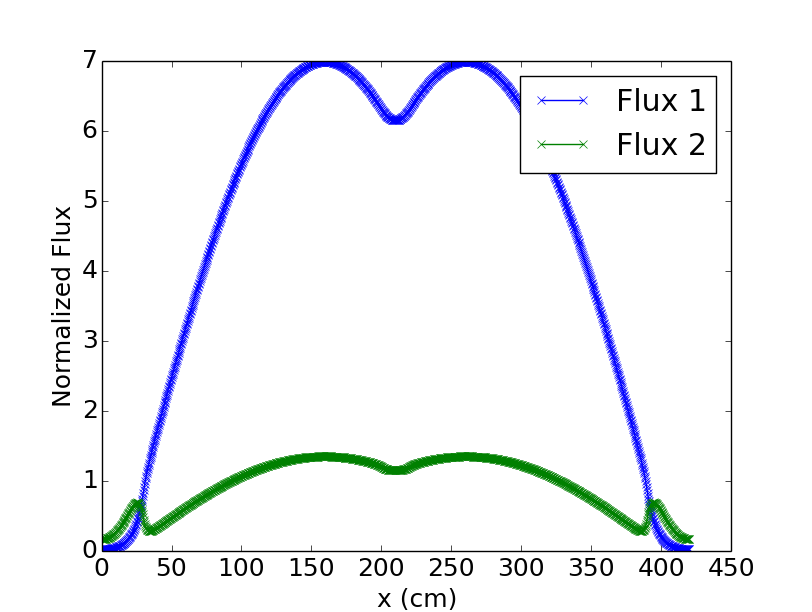
\includegraphics[width=.9\linewidth]{rod_flux.png}
				\caption{Rodded Core}
				\label{fig::rod_flux}
			\end{subfigure}%
			\begin{subfigure}{.5\textwidth}
				\centering
				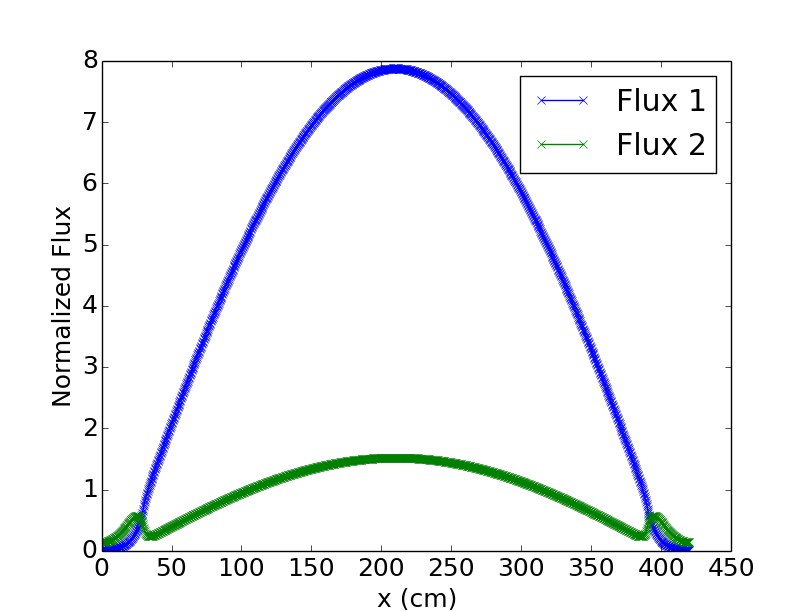
\includegraphics[width=.9\linewidth]{urod_flux.png}
				\caption{Unrodded Core}
				\label{fig::urod_flux}
			\end{subfigure}
			\caption{Fast and thermal flux profiles for 1D reactor core problems solved with a fine mesh.}
			\label{fig::flux_profiles}
		\end{figure}	
	
	Notice that the presence of the rod material greatly suppresses the flux in the center of the core where the flux is naturally greatest without the presence of the rod. To determine the spatial convergence of these problems, we define nodes over which the fission source is averaged. Each node can contain multiple mesh points. 
	
	We define all errors relative to the solution with the finest mesh spacing. The error $\epsilon_{k,c}$ in k-effective for a computed eigenvalue $k_c$ is defined as
	\begin{equation}
	\epsilon_{k,c} = \frac{k_c - k_\text{ref}}{k_\text{ref}}
	\end{equation}
	where $k_\text{ref}$ is the computed eigenvalue for the reference fine mesh solution. The error in nodal power $\epsilon_{p,c}$ for a computed fission distribution $f_c(x)$ is defined by the RMS error relative to the reference nodal fission distribution $f_\text{ref}(x)$ as
	\begin{equation}
	\epsilon_{p,x} = \sqrt{\frac{1}{N} \sum_{n=1}^N \left( \frac{f_c(x_n) - f_\text{ref}(x_n)}{f_\text{ref}(x_n)} \right)^2}
	\end{equation}
	where $N$ is the number of nodes. In Fig.~\ref{fig::spatial_convergence} the errors in k-effective and the fission source are plotted against the number of mesh points per node for both the rodded and unrodded cores. 
	
	
			\begin{figure}[ht]
				\centering
				\begin{subfigure}{.5\textwidth}
					\centering
					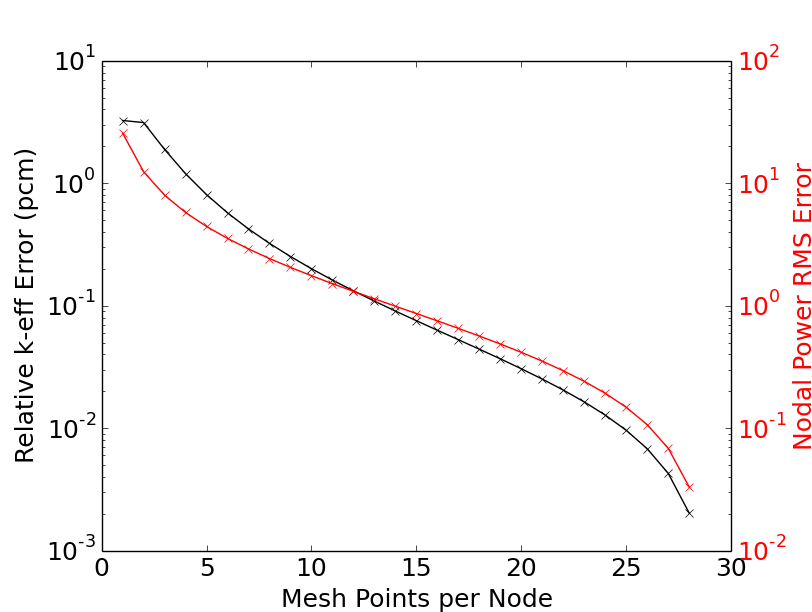
\includegraphics[width=.9\linewidth]{log_mesh_refinement_errors.png}
					\caption{Rodded Core}
					\label{fig::rod_sp_conv}
				\end{subfigure}%
				\begin{subfigure}{.5\textwidth}
					\centering
					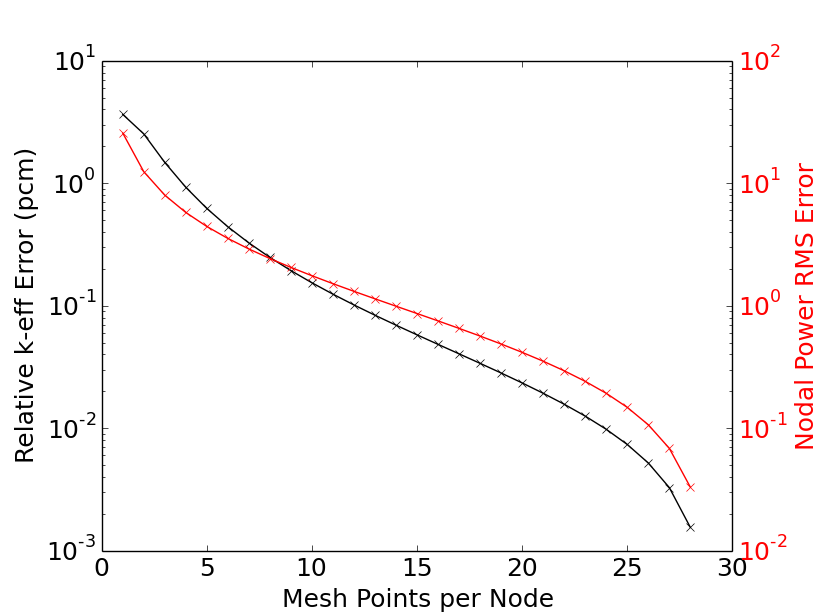
\includegraphics[width=.9\linewidth]{urod_log_mesh_refinement_errors.png}
					\caption{Unrodded Core}
					\label{fig::urod_sp_conv}
				\end{subfigure}
				\caption{Spatial convergence of 1D core showing errors in k-effective and nodal power against the number of mesh points per node.}
				\label{fig::spatial_convergence}
			\end{figure}
	
	Notice that in both the rodded and unrodded cases, k-effective converges faster than nodal power.
		
	\clearpage
	\paragraph{Part C: Dominance Ratio}
	When the eigenvalue is computed, the most common approach is to use the power method. This simple method for computing the largest eigenvalue of a matrix converges geometrically as
	\begin{equation}
	\epsilon_{i+1} = D \epsilon_{i}
	\end{equation}
	where $\epsilon_i$ refers to the error in iteration $i$. $D$ denotes the dominance ration which is defined by
	\begin{equation}
	D = \left| \frac{\rho_2}{\rho_1} \right|
	\end{equation}
	where $\rho_1$ is the largest eigenvalue and $\rho_2$ is the second largest eigenvalue. Therefore, for fast convergence, we would like for $\rho_2 << \rho_1$. However, this is rarely the case in realistic reactor physics problems. To make matters worse, the dominance ratio increases as the mesh is refined. This phenomenon is shown in Fig.~\ref{fig::dr} for both the rodded and unrodded 1D reactor core problems. Note that for both cases the dominance ratio is greater than 0.99 and the rodded case has a slightly higher dominance ratio than the unrodded case. This is because the rodded case has greater contribution from other eigenmodes as the flux profile is more complex.
	
			\begin{figure}[ht]
				\centering
				\begin{subfigure}{.5\textwidth}
					\centering
					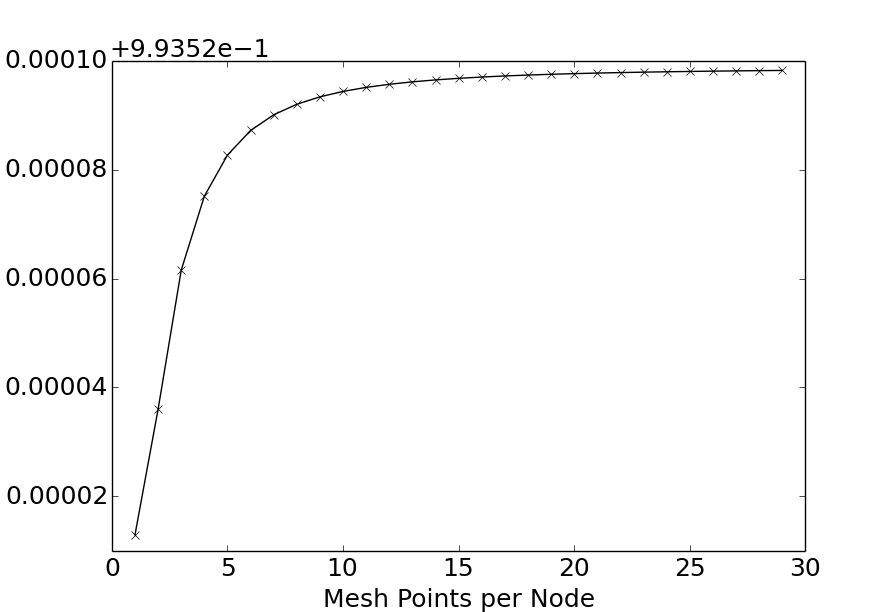
\includegraphics[width=.9\linewidth]{DR.png}
					\caption{Rodded Core}
					\label{fig::rod_dr}
				\end{subfigure}%
				\begin{subfigure}{.5\textwidth}
					\centering
					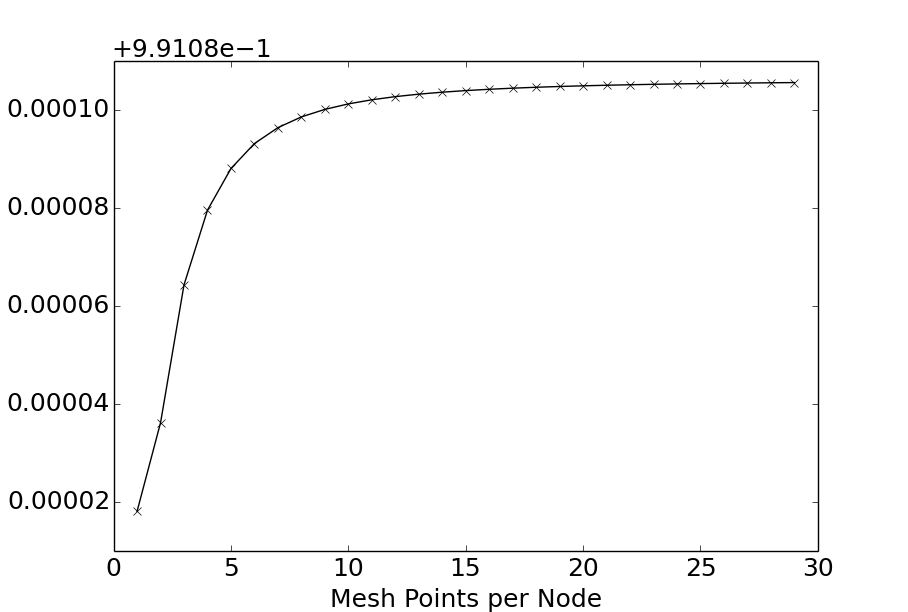
\includegraphics[width=.9\linewidth]{urod_DR.png}
					\caption{Unrodded Core}
					\label{fig::urod_dr}
				\end{subfigure}
				\caption{Dominance ratios of 1D reactor core problems increasing with mesh refinement.}
				\label{fig::dr}
			\end{figure}
				
	\paragraph{Part D: Point Jacobi}
	During each iteration of the power method, a linear system needs to be solved of the form
	\begin{equation}
	A \phi_\text{new} = F \phi_\text{old}
	\end{equation}
	for $\phi_\text{new}$ using the previous solution $\phi_\text{old}$. This takes the form of a simple $Ax = b$ where $b = F\phi_\text{old}$. One method used to solve $Ax = b$ is the Point Jacobi method. 
	
	In this general method, the matrix $A$ is decomposed into three parts - lower triangular elements $L$, diagonal elements $D$, and upper triangular elements $U$. Therefore,
	\begin{equation}
	A = L + D + U.
	\end{equation}
	In the Point Jacobi method, we solve
	\begin{equation}
	(L+U)x_{i+1} = b-D^{-1} x_i 
	\end{equation}
	where $x_i$ refers to the solution vector at iteration $i$. This method is guaranteed to converge if
	\begin{equation}
	\left|A_{ii}\right| > \sum_{j \neq i} \left|A_{ij}\right|.
	\end{equation}
	
	To determine the impact of convergence tolerance on the solver, the convergence tolerance of the power method is fixed at $10^{-6}$ on the fission source, but the flux convergence on the inner Point Jacobi solution is varied. The result is shown in Fig.~\ref{fig::PJ_convergence}.
			\begin{figure}[ht]
				\centering
				\begin{subfigure}{.5\textwidth}
					\centering
					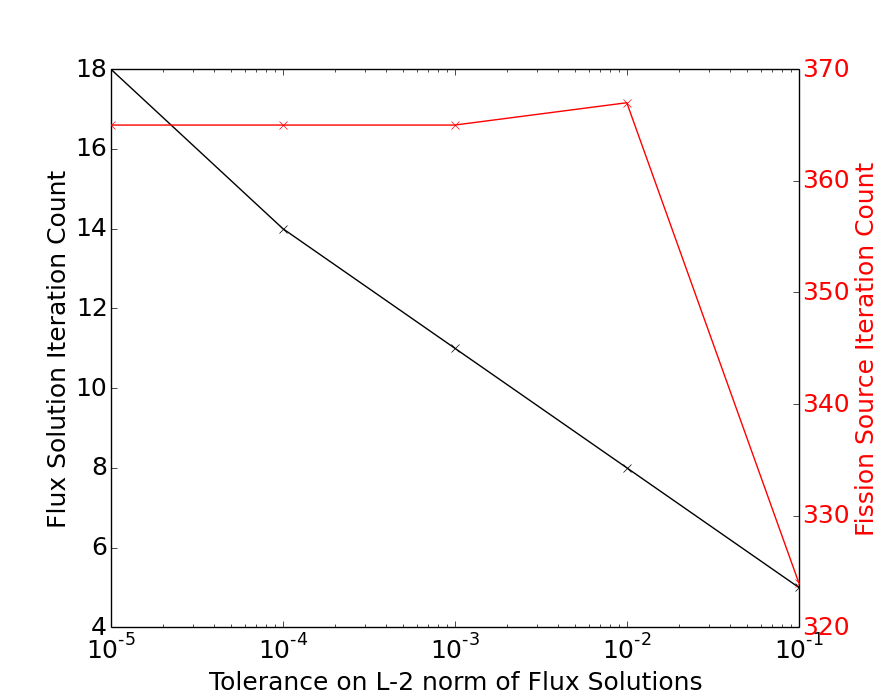
\includegraphics[width=.9\linewidth]{rod_PJ.png}
					\caption{Rodded Core}
					\label{fig::rod_pj}
				\end{subfigure}%
				\begin{subfigure}{.5\textwidth}
					\centering
					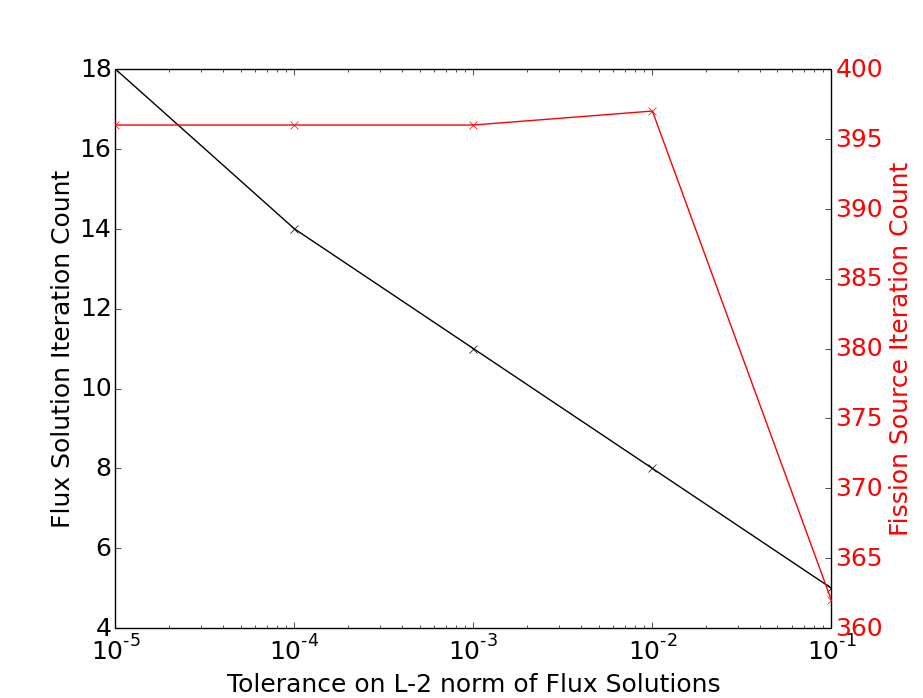
\includegraphics[width=.9\linewidth]{urod_PJ.png}
					\caption{Unrodded Core}
					\label{fig::urod_pj}
				\end{subfigure}
				\caption{Number of iterations required to converge 1D reactor problems using the Point Jacobi method to solve the Flux.}
				\label{fig::PJ_convergence}
			\end{figure}	
			
	Notice that, as expected, the number of Point Jacobi iterations increases as the tolerance is tightened. However, notice that after a sufficient tightening of the tolerance, the number of required fission source iterations remains constant. 
	
	At extremely loose tolerance on the flux, the number of iterations plummets. This is most likely due to the Point Jacobi method producing a solution that is incorrect but the difference between the previous iteration is sufficiently small. Therefore, the loosely converged flux causes the final flux solution to be incorrect. 
	
	\paragraph{Part E: Gauss-Seidel}
	An alternative method to solve a linear system of the form $Ax = b$ is the Gauss-Seidel method. This method is very similar to Point Jacobi, except updated solution vector values from the current iteration are used in the multiplication with the lower diagonal elements. More specifically, the algorithm is transformed so that we solve
	\begin{equation}
	Ux_{i+1} = b-(L+D)^{-1} x_i.
	\end{equation}
	The Gauss-Seidel method typically has a faster convergence since it is using more updated information. The same trials are conducted on the convergence as with Point Jacobi and the results are presented in Fig.~\ref{fig::GS_convergence}.
				\begin{figure}[ht]
					\centering
					\begin{subfigure}{.5\textwidth}
						\centering
						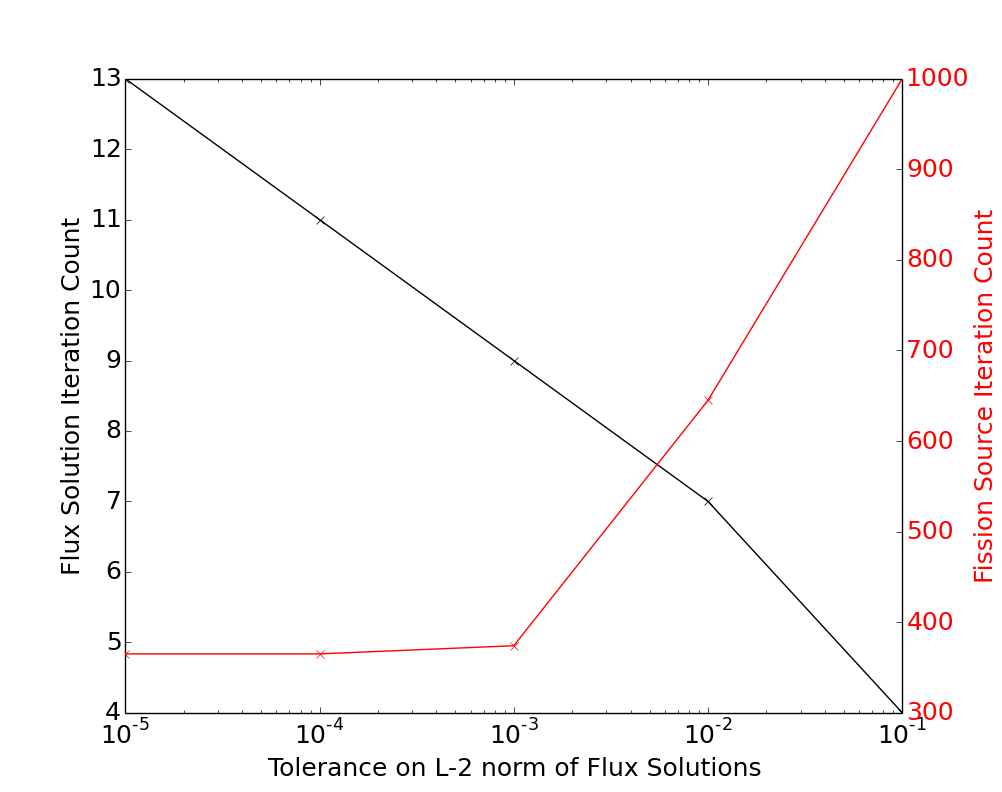
\includegraphics[width=.9\linewidth]{rod_GS.png}
						\caption{Rodded Core}
						\label{fig::rod_gs}
					\end{subfigure}%
					\begin{subfigure}{.5\textwidth}
						\centering
						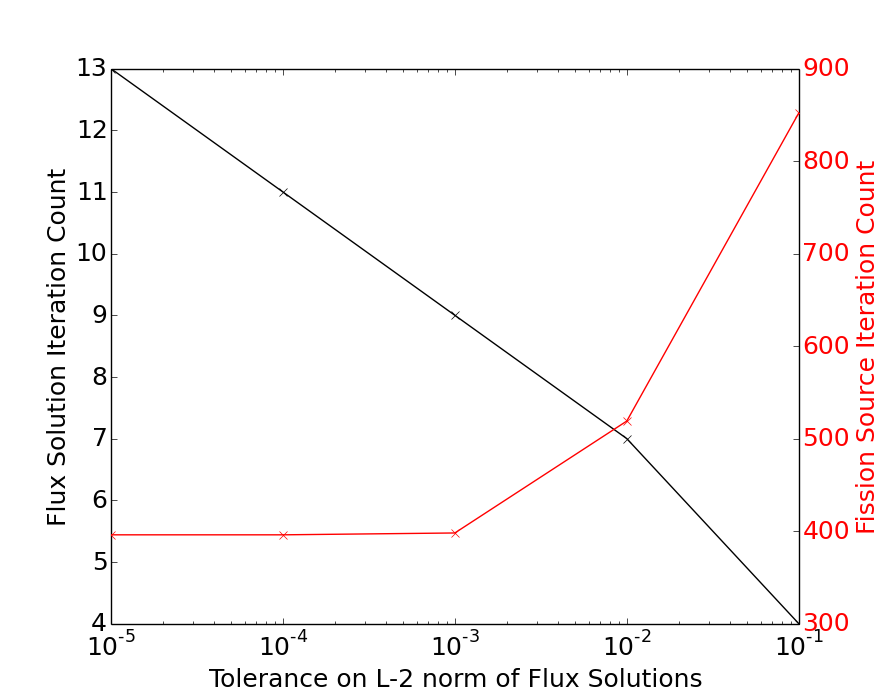
\includegraphics[width=.9\linewidth]{urod_GS.png}
						\caption{Unrodded Core}
						\label{fig::urod_gs}
					\end{subfigure}
					\caption{Number of iterations required to converge 1D reactor problems using the Gauss-Seidel method to solve the Flux.}
					\label{fig::GS_convergence}
				\end{figure}
	
	As before, we see that as the convergence criteria is tightened, the number of required Gauss-Seidel iterations increases as expected. Also, we notice that once the convergence criteria is tight enough, the number of required fission source iterations to converge the solution remains relatively constant. 
	
	However, notice at loose convergence criteria we observe a trend opposite of that observed with Point Jacobi. This is because Gauss-Seidel is able to deliver far more accurate estimates of the flux at lower iteration counts due to the more rapid transfer of updated information. Therefore, instead of converging to an incorrect solution, Gauss-Seidel attempts to converge to the correct solution. As the convergence iteration criteria is loosened, the number of fission source iterations seems to increase exponentially as the eigenvalue solver suffers from inaccurate estimates of the scalar flux.
	
	Notice that in both the Point Jacobi and Gauss-Seidel solvers, the rodded core required greater iteration counts. This is because the unrodded core is relatively simple with a more dominant main eigenmode (lower dominance ratio).
	
	\paragraph{Part F: Real and Adjoint Fluxes}
	Earlier in Fig.~\ref{fig::flux_profiles}, the real scalar flux was plotted for both groups 1 and 2 for the rodded and unrodded problems. The eigenvalues corresponding to these problems are presented below in Table~\ref{tab::eigenvalues}.

	\begin{table}[ht]
		\begin{center}
			\caption{\label{tab::eigenvalues} Dominant eigenvalues of 1D reactor problems}
			\begin{tabular}{ll}
				\hline
				Rodded & Unrodded \\
				\hline
				1.3646153 & 1.3680008 \\
				\hline
			\end{tabular}
		\end{center}
	\end{table}
	
	As expected, the unrodded eigenvalue is higher. Many times we are also interested in the solution to the adjoint problem,
	\begin{equation}
	A^T \phi^* = \frac{1}{k^*} F^T \phi^*.
	\end{equation}
	The solution $\phi^*$ is the adjoint flux which describes the neutron importance and $k^*$ is the eigenvalue of the adjoint problem. $A^T$ denotes the transpose of the loss matrix and $F^T$ denotes the transpose of the fission matrix. Remembering Eq.~\ref{eq::matrix}, we can multiply the real version of the matrix equations by the transpose of the adjoint flux, yielding
	\begin{equation}
	\left(\phi^*\right)^T A \phi = \frac{1}{k} \left(\phi^*\right)^T F \phi.
	\end{equation}
	Transposing both sides of the equation, we find
	\begin{eqnarray}
	\left(\left(\phi^*\right)^T A \phi \right)^T= \left(\frac{1}{k} \left(\phi^*\right)^T F \phi \right)^T \\
	\phi^T A^T \phi^* = \frac{1}{k} \phi^T F^T \phi^* \\
	\phi^T \left(A^T \phi^* \right) = \phi^T \left(\frac{1}{k} F^T \phi^* \right) \\
	A^T \phi^* = \frac{1}{k} F^T \phi^*
	\end{eqnarray}
	Therefore $k^* = k$, meaning that the eigenvalues computed from the real and adjoint problems should be identical. This is indeed observed as the values presented in Table~\ref{tab::eigenvalues} are reproduced for the adjoint solution.
	
	The from the values presented in Table~\ref{tab::eigenvalues} we can also determine the static rod worth. To calculate the rod worth $\rho_r$, we apply the equation
	\begin{equation}
	\rho_r = \frac{k_\text{urod} - k_\text{rod}}{k_\text{urod} k_\text{rod}}
	\end{equation}
	where $k_\text{urod}$ refers to the eigenvalue of the solution without the rod and $k_\text{rod}$ refers to the solution with the rod inserted. Using this equation, a rod worth of \textbf{181 pcm} is calculated.
	
	The adjoint flux solution is plotted in Fig.~\ref{fig::adj_flux} for both the rodded and unrodded cases. 
	
			\begin{figure}[ht]
				\centering
				\begin{subfigure}{.5\textwidth}
					\centering
					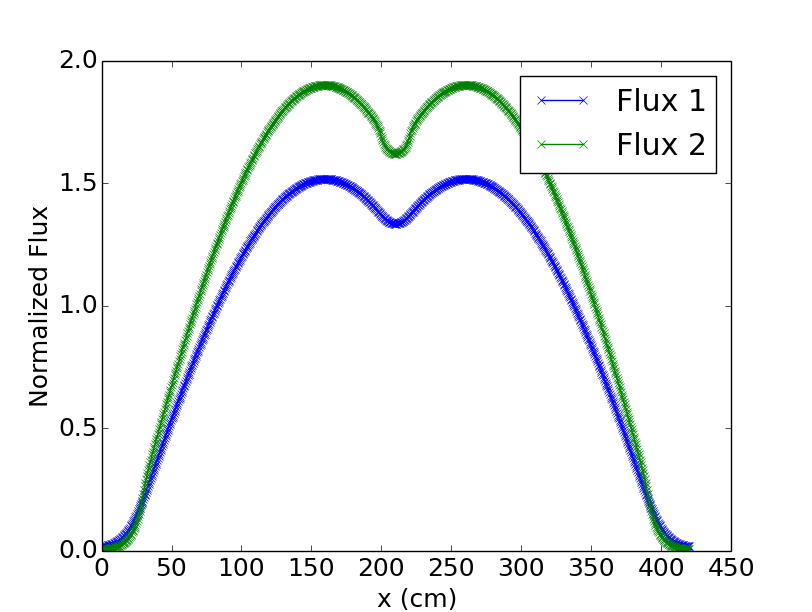
\includegraphics[width=.9\linewidth]{rod_adjoint_flux.png}
					\caption{Rodded Core}
					\label{fig::rod_adj_flux}
				\end{subfigure}%
				\begin{subfigure}{.5\textwidth}
					\centering
					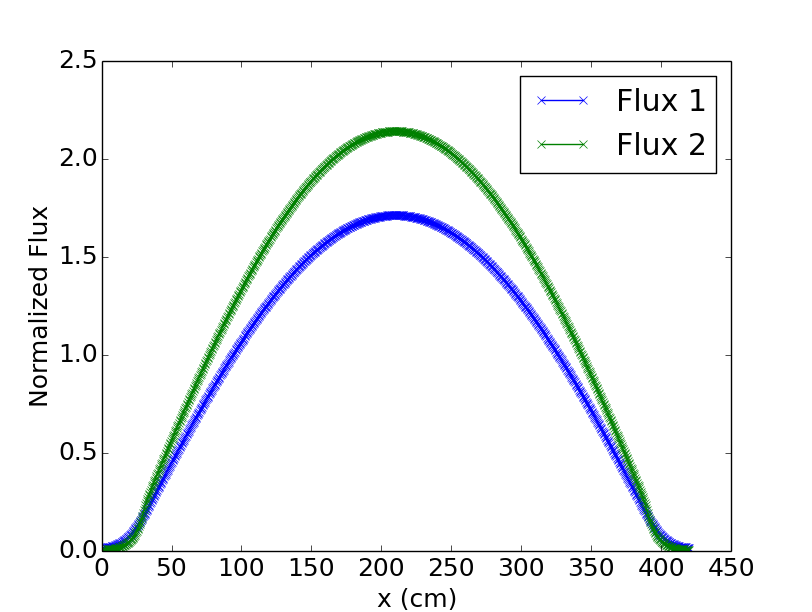
\includegraphics[width=.9\linewidth]{urod_adjoint_flux.png}
					\caption{Unrodded Core}
					\label{fig::urod_adj_flux}
				\end{subfigure}
				\caption{Fast and thermal adjoint flux profiles for 1D reactor core problems solved with a fine mesh.}
				\label{fig::adj_flux}
			\end{figure}
			
	Notice that the solutions are very similar to the real flux profiles presented in Fig.~\ref{fig::flux_profiles}. However, there are some slight differences. In general, the adjoint flux profile is far less peaked. This is because neutrons sufficiently far in the fuel should have around the same importance. As the 1D reactor is more than 400 cm in width, its width is far greater than the mean neutron flight path. Intuitively, a neutron 100 cm into the core should have approximately the same importance as a neutron 200 cm into the core as both have approximately the same probability of causing a fission even though the neutron flux is much higher in the center of the core. 
	
	In addition, the adjoint flux depression is much steeper in the rodded material as neutrons traveling through the rodded material have a much reduced chance of initiating a fission event before being absorbed.
	
	
\end{document}